% example.tex: LaTeX example annual report
\documentclass[11pt]{article}
\usepackage{fullpage}
\usepackage{courier}
\usepackage{graphicx}
\usepackage{floatrow}
\usepackage{amsmath}
\usepackage{amssymb}
\usepackage{centernot}

\begin{document}
%---------------------------------------------------
\title{\Large \bf Cache Efficient Sort and List Ranking}
\author{Avesh Singh \and Grant Strimel}

\maketitle
%----------------------------------------------------
\section{Introduction}
This section's conte


\section{I/O Model}
The standard theoretical model for analyzing algorithms is known as the the \textit{Ram Model}.
The model assumes an infinitely sized memory with a uniform cost for each access.  An algorithm's efficiency is then 
evaluated in this model by the number of operations between variables and pieces of memory performed during execution. 
Though theoreticall valid when ..., the model is not sufficient to capture hierarchical nature and locality sensitives of the memory 
system in a real computer system.

A real modern computer often has many ``cacheing" layers for memory access.  Layers which are closer to the CPU, 
like the L1 and L2 caches, are small in size and cost less for accesses. Caches which further down in the hierarchy, such as 
main memory and hard drive, are much larger but are expensive to access.  The I/O-model attempts to capture the cost of accesses 
in a stucture with varying expenses.

Formally, the I/O model abstracts a single level system.  There is a chache of size $M$ (contains $M$ objects).  
Accessing an element/location which is currently in the cache is a free operation.  The cache is broken down by blocks or 
cache lines of size $B$ which are simply contiguous blocks of memory (the cache has $M/B$ blocks).  
When accessing an element which is currently not in 
cache, block transer between the cache and ``slow memory" (file system)  must occur.  The transfer requires I/O operations, 
a write of the evicted block and the read of the block being loaded.  This block transer has a cost of $O(1)$.  Hence 
analyzing algorithms in the I/O model is matter of asymtotically bounding the number of blocks transfers.  
Figure \ref{theiomodel} below illustrates the I/O model.

\begin{figure}[H]  
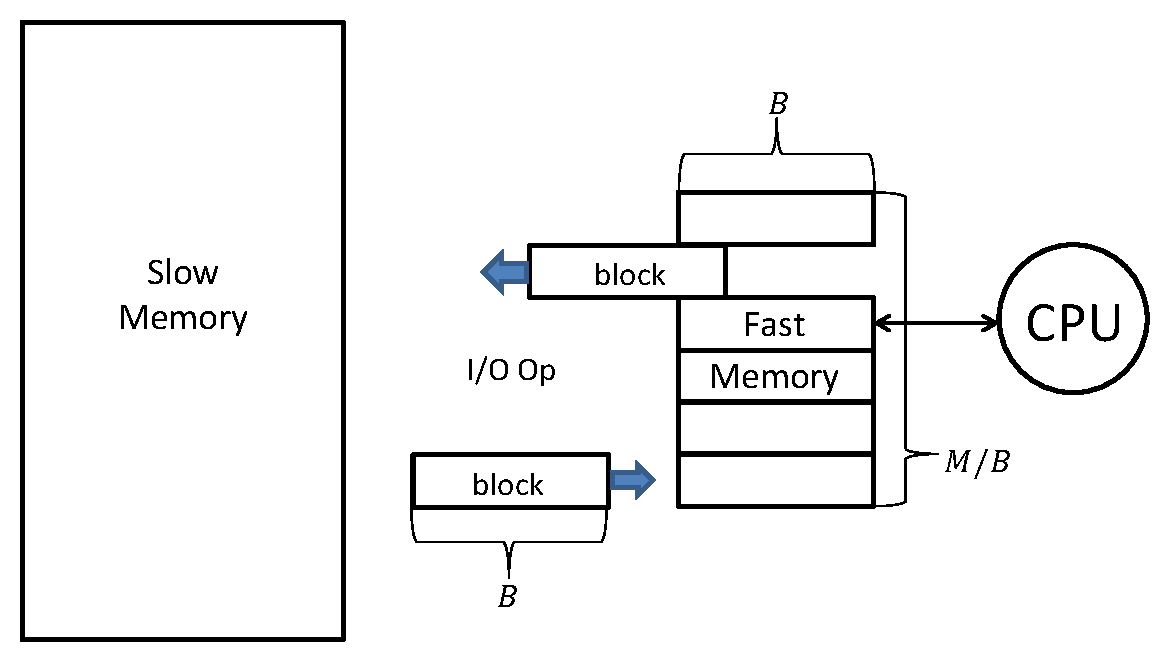
\includegraphics[scale=0.5]{figures/iofsfig.pdf}
\caption{the I/O Model}
\label{theiomodel}
\end{figure}

For our project we implemented an I/O cache object (\texttt{LRUCache}) to emperically study algorithms under a single level cache.
 The class at its core implements  LRU cache which interacts with the file system.  The cache takes as parameters a block size 
$B$ and and the number of elements it can contain at one time $M$.  
The \texttt{LRUCache} can instatiate two types of objects: \texttt{FileCacheArray<T>} and 
\texttt{EmptyCacheArray<T>}.  These objects act exactly like arrays or lists with \texttt{get} and \texttt{set} methods, however 
behind the scenes the \texttt{LRUCache} is handling all IO operations.  On cache misses, it loads the approporite block from file 
inserts it into the cache and sinultaneiously the block that is evicted is written to its appropriate file.  The difference between 
\texttt{FileCacheArray<T>} and \texttt{EmptyCacheArray<T>} is that \texttt{FileCacheArray<T>} is inniated with an existing file 
specified and filled with that file's contents while \texttt{EmptyCacheArray<T>} only takes a size and does not guarentee the initial 
contents of the array.

The cache most importantantly keeps counts \textit{accesses}, \textit{hits}, and \textit{misses} accross all arrays.  Thus we are 
able to analyze an I/O algorithm using our customized data strucutres emperically by comparing these statistics on 
termination. 


\section{Cache Efficient Sort}

\subsection{Algorithm Descriptions}


We implemented an IO Efficient Mergesort, using a k-way merge. We describe the algorithm below.

We first split the input array into k subarrays and sort each recursively

%% , and then perform a k-way merge. We set k equal to (number of blocks)/2.

Then we merge the k subarrays in the same way as a standard mergesort, except that we store a pointer for each subarray and take the largest element at the pointer within each subarray and insert this into a sorted copy of the array. After we have copied all elements from the sorted subarrays into the copy, we replace the original array with the sorted copy.

To perform efficiently in an IO model, we set k equal to (number of blocks)/2. In the merge step we keep only one block in memory per subarray, and so we have enough cache blocks for the subarrays, the copied output array, and the array of pointers into the subarrays. 

Note that it may be equally efficient to set k equal to (number of blocks) - 1 - k/(block size), since we need to keep only one block at a time in memory for the copied array, and require approximately k/(block size) blocks to store the array of pointers. In order to not hassle with small additive constants on the space requirement, we decided to use the above, lower k value.

In analyzing the complexity of our IO Efficient Mergesort, let N be the number of elements to sort, B the block size, and M the total cache size.

In the base case of the IO Efficient Mergesort, we can sort in memory for free, so the cost is $\theta(M/B)$

In the merge step, we can have $\theta(N/B)$ cache misses since we retrive the blocks of the subarrays iteratively.

Thus our recurrence is:

\begin{align*}
S(N) = (M/B)S(NB/M) + \theta(N/B) \\
\text{and so} \\
S(N) = \theta((N/B)(log_{M/B}(N/M) +1))
\end{align*}

In order to evaluate the efficiency of our IO Efficient Mergesort, we also wrote Quicksort and Selection Sort.

We implemented these algorithms in Java using the following classes: \texttt{IOEfficientMergeSort}, \texttt{QuickSort}, and \texttt{SelectionSort}.

\section{Sorting Experiments}

\subsection{Performance Comparison}

\begin{figure}[H]  
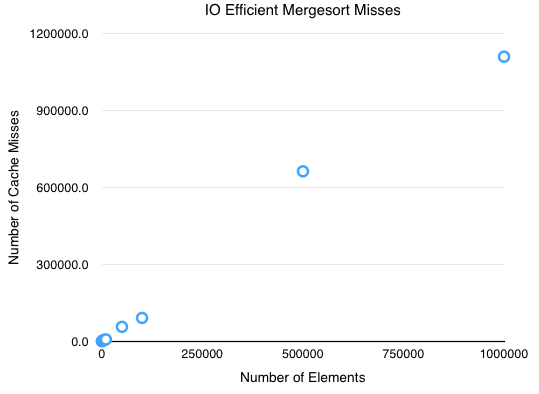
\includegraphics[scale=0.6]{figures/IOEfficientMisses.png}
\caption{IO Efficient Mergesort}
\label{listrankingio}
\end{figure}

\begin{figure}[H]  
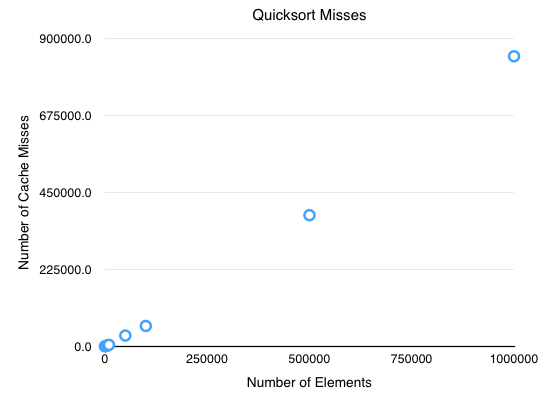
\includegraphics[scale=0.6]{figures/QuicksortMisses.png}
\caption{Quicksort Misses}
\label{listrankingio}
\end{figure}

\begin{figure}[H]  
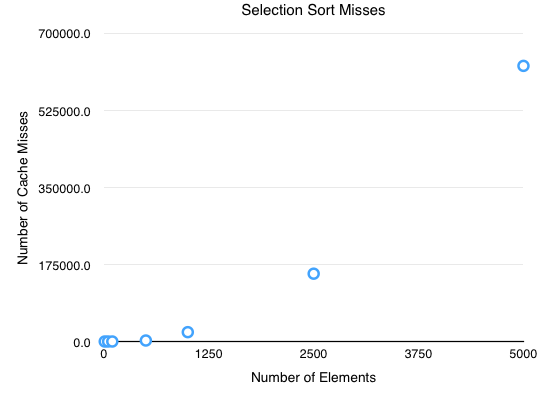
\includegraphics[scale=0.6]{figures/SelectionSortMisses.png}
\caption{Selection Sort Misses}
\label{listrankingio}
\end{figure}

The constant factor for IO Efficient Mergesort is higher than that of Quicksort. Because of this, these two algorithms perform similarly on small input. The graph of IO Efficient Mergesort Misses, however, is concave --the number of cache misses is leveling off. The graph of Quicksort Misses, however, is convex --the number of cache misses will increase significantly on larger numbers of elements.

It is clear that the selection sort is performing far worse than IO Efficient Mergesort. For 5000 elements, we have 600,000 misses. In the IO Efficient sort, we have only 4500 misses.

Because of the overhead of our cache simulator, we were not able to run simluations with more than 1,000,000 elements.

\subsection{Varying Blocksize}

\begin{figure}[H]  
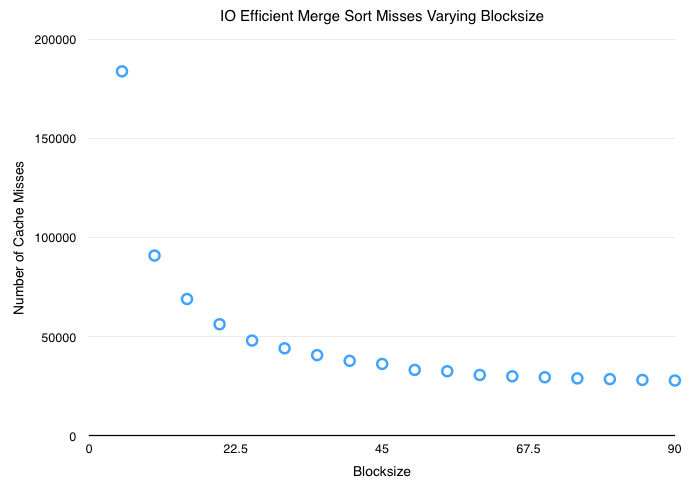
\includegraphics[scale=0.45]{figures/Blocksize_IOEfficientMergeSort.png}
\caption{Selection Sort Misses}
\label{listrankingio}
\end{figure}

\subsection{Varying Number of Blocks}

\begin{figure}[H]  
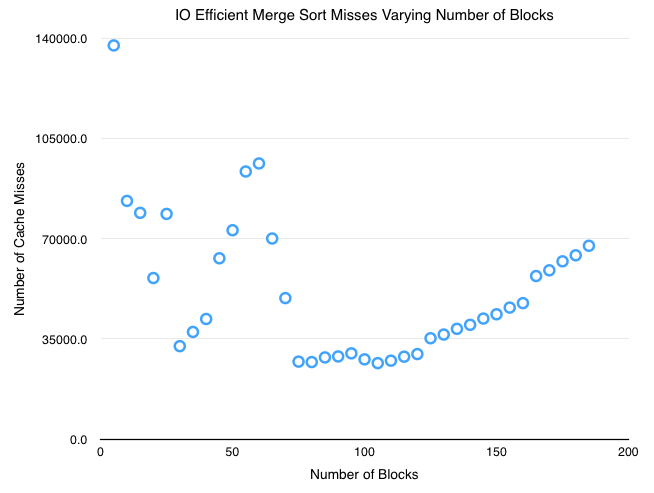
\includegraphics[scale=0.45]{figures/NumBlocks_IOEfficientMergeSort.png}
\caption{Selection Sort Misses}
\label{listrankingio}
\end{figure}


\section{Cache Efficient List Ranking}
Some problems which have very natural solutions in the standard model can have significant more complexity in the I/O Model. 
Many of these problems involve pointer based algorithms.  Since pointers can potentially point to any memory location, without 
taking care an algorithm can easily start incurring many consecutive block misses, drastically increasing I/O complexity.  One 
such example is the problem known as list ranking.  List ranking asks given a linked list presented in an array in memory, determine 
the position of each node and label in accordingly.  See Figure  \ref{listrankingio}.

\begin{figure}[H]  
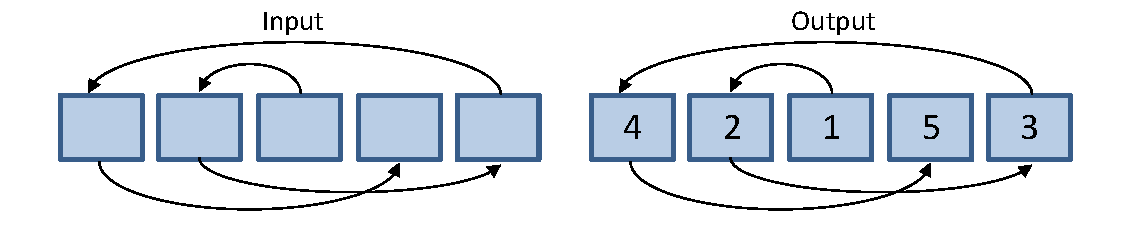
\includegraphics[scale=0.5]{figures/listrankingio.pdf}
\caption{List Ranking Problem}
\label{listrankingio}
\end{figure}

An approach which runs $O(n)$ in the standard complexity model and is optimal in the model is to simply scan the list to determine the 
starting node, and then simply hop from node to node while incrementally increaseing the label.  This however is a naive approach in 
the I/O model.  The complexity is the worst case is $O(n)$ since the list could be constructed in such a way that a cache miss is incurred on 
every ``hop".  The algorithm does not account for locality.  

We can improve on this run time by taking advantage of our I/O efficient.  Effectively the improved algorithm will run in $O(sort(n))$. 

\subsection{Algorithm Description}


\begin{enumerate}
  \item Indentify independent set
  \item Bridge out
  \item Recurse on subproblem
  \item Merge result
\end{enumerate}

\subsubsection{Independent Set}
Indentify the independent set requires flipping a coin for each node.  A node is in the independent set if the coin was heads for 
it while tails for its predecessor. Thus by linearity of expectation, on average a fourth of the nodes will be in the set. 
This can be done efficient by flipping the coin for each node, copying the the list then sorting the copy 
by successor address. Then the lists can simply be scan simulatneous checking corresponding positions for the correct criteria.  This step 
requires some scans and a sort and thus runs in $O(sort(n))$. 

\subsubsection{Bridge out}
After the independent set is identified, the nodes it contained be removed from the list so that that a smaller subproblem can be recursed on.
This is called bridgeing out.  Each independent set node most set its predecessor to point over it to its successor. A special edge 
with additional weight should be used to mark the number of nodes the bridge is skipping over.  In the singly linked list application this 
requires two copies and two sorts by successor address.  One can then align/stack the lists and scan over them putting a ``bridge" in place 
where neccessary.  This step is again bounded by $O(sort(n))$.

\subsubsection{Recurse on subproblem}
Once we bridge out the independent set we have a smaller subproblem we can recurse on.  When the list becomes of a size which can fit in cache, we can then run standard pointer hopping algorithm since all operations are now free once the data is loaded to the cache.

\subsubsection{Merge result}
After solving the subproblem, we must take the results and fill in the missing ranks of the independent set.  This can be done rather easily 
by using another sort and a few scans.

Hence the the running time can be expressed as teh following recurrence; $R(n) = R(n/c) + O(sort(n)) \in O(sort(n))$.

\section{Ranking Simulations}

We implemented both the standard list ranking (\texttt{ListRanking.rankListNaive}) procedure and the cache efficient version
 (\texttt{ListRanking.rankList}) in Java utilizing our \texttt{LRUCache} to emperically test the 
efficiency of  both methods.  We ran both methods on randomly permuted lists and compared the cache misses of each.  

Figure \ref{naivelistranking} shows the naive method's performance in terms of cache misses.  As is expected the algorithm has misses which is almost linear with the number of nodes in the list.

\begin{figure}[H]  
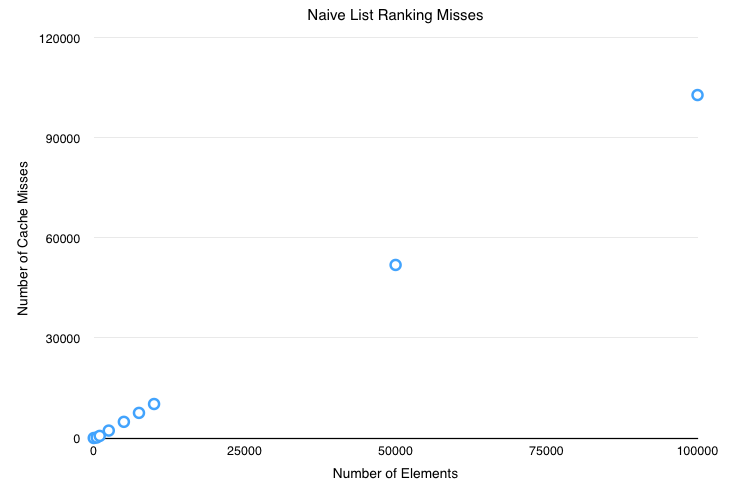
\includegraphics[scale=0.5]{figures/NaiveListRanking.png}
\caption{Naive List Ranking}
\label{naivelistranking}
\end{figure}

As you can see there are more misses initially but the graph is leveling off as the number of elements in the list grows larger.  This behavior is 
as expected since as $n$ becomes sufficiently large and can no longer fit in memory, the algorithm which utilizes locality more does better.

\begin{figure}[H]  
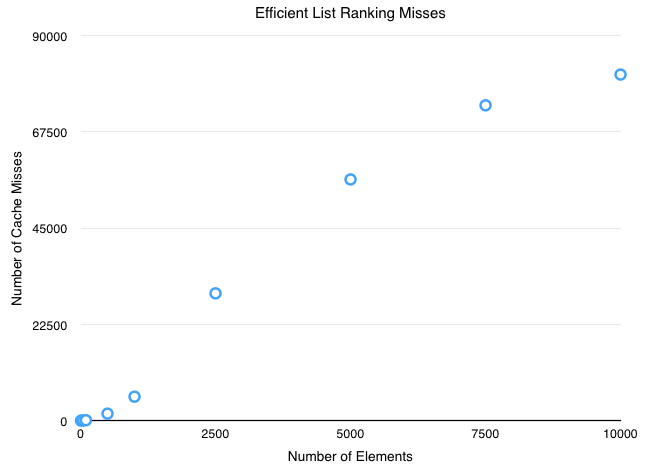
\includegraphics[scale=0.5]{figures/EfficientListRanking.png}
\caption{Efficient List Ranking}
\label{efficientlistranking}
\end{figure}


\end{document}
